\section{Introduction}

Personality is a comprehensive yet complex trait that encapsulates individual differences in patterns of thinking, feeling, and behaving~\citep{article}. Detecting personality automatically is of significant importance for improvement of machine's ability to have human-like cognition and engage in more natural interactions with humans, particularly in the context of advancing Artificial General Intelligence (AGI) and various practical applications such as reflective linguistic programming~\citep{fischer2023reflective}, disease diagnosis~\citep{6709853} and mental health prediction~\citep{feng2024far}. In recent years, there has been a burgeoning interest in automatic personality detection, marking a significant shift from traditional methods to innovative computational approaches. 
At the very beginning, owing to the limitations of multimedia model and computational power, researchers only treat personality prediction as a straightforward text classification task, aiming to decipher personality traits from the digital footprints individuals leave online~\citep{kerz2022pushing,yang_multi-document_2021}. However, as shown in Figure \ref{fig:example}, researchers have increasingly recognized that personality is manifested via multi-dimensions, with nuances that pure text-based analysis cannot fully capture~\citep{10.1145/3542954.3543012,ijcai2022p633,10030882}. This revelation has propelled the move towards multimodal personality detection as the mainstream methodology.
\begin{figure}[th]
  \centering
  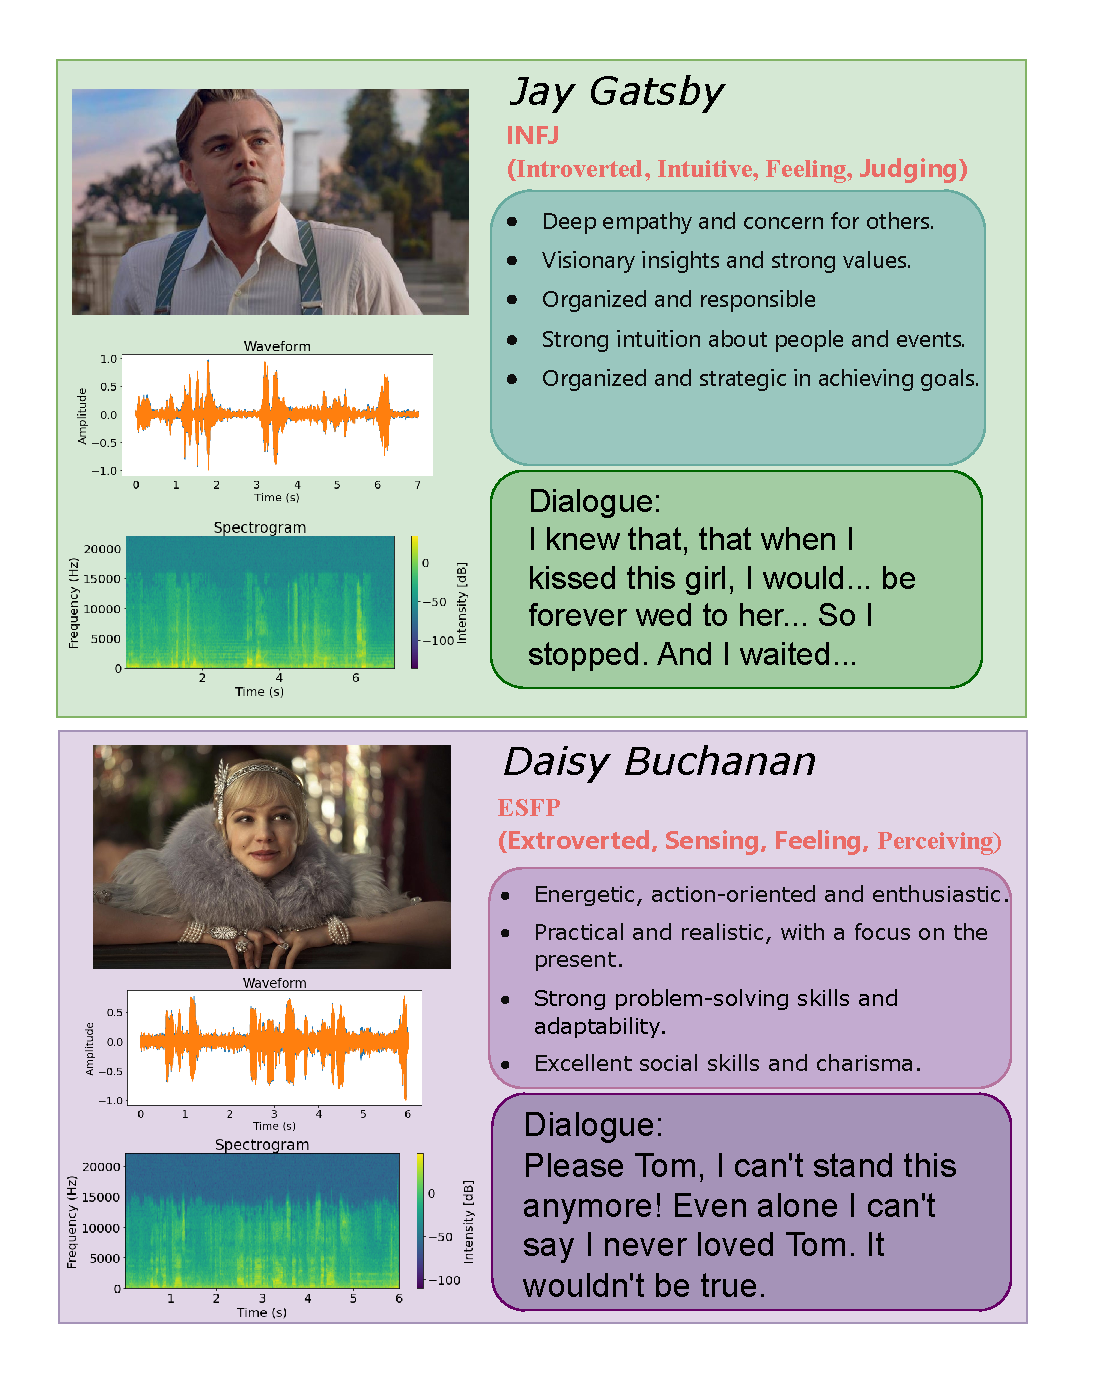
\includegraphics[width=\linewidth]{images/example.pdf}
  \caption{The Distinctive Features in Three Modalities for Personality Prediction}
  \label{fig:example}
\end{figure}

% \begin{figure}[ht]
%   \centering
%   % First subfigure
%   \begin{subfigure}[b]{\textwidth}
%       \centering
%       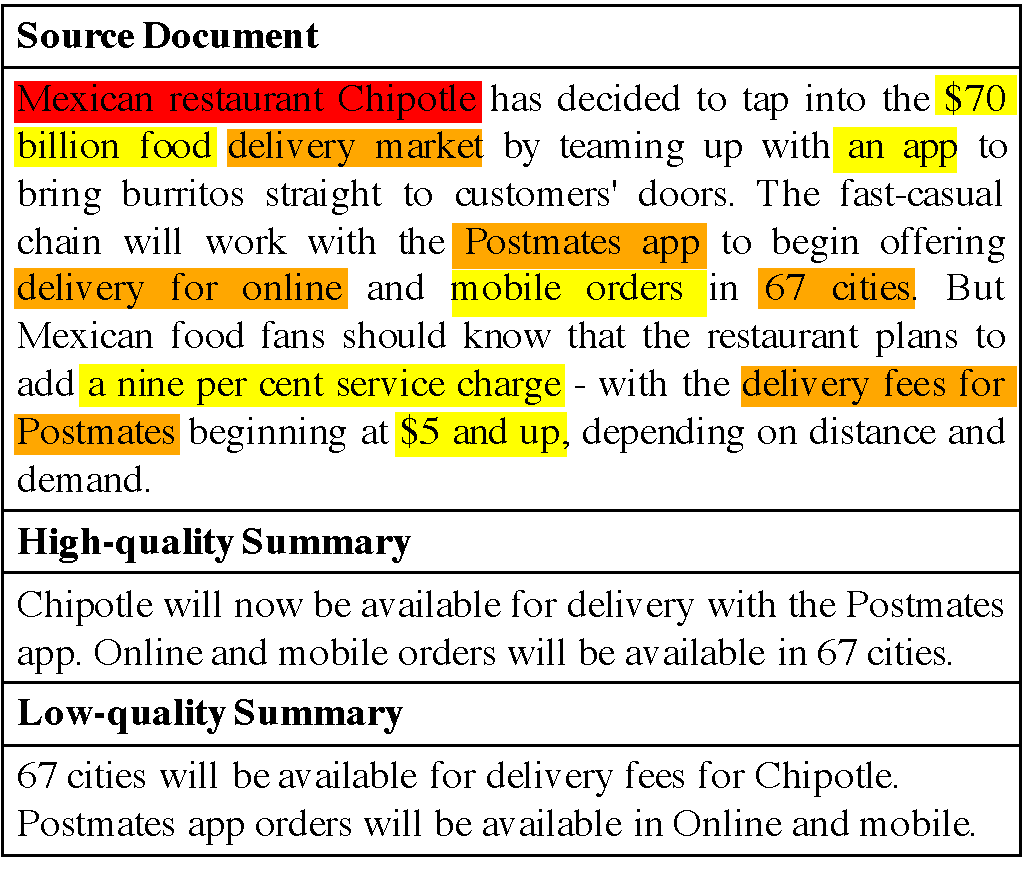
\includegraphics[width=\textwidth]{images/example1.pdf}
%       \label{fig:first}
%   \end{subfigure}
  
%   % Second subfigure
%   \begin{subfigure}[b]{\textwidth}
%       \centering
%       
\includegraphics[width=\textwidth]{images/example2.pdf}
%       \caption{Caption for second graph}
%       \label{fig:second}
%   \end{subfigure}
  
%   \caption{The Distinctive Features in Three Modalities for Personality Prediction}
%   \label{fig:combined}
% \end{figure}

Personality datasets, integrating text, audio, visual information along with the manner of speaking, face expressions, body language and so on, offer a richer, more nuanced view of human behavior and personality expressions than text-based datasets alone. This comprehensive approach is essential for developing models that accurately reflect the complexity of human personality. Naturally, a lot of multimodal datasets were released in recent years. There have been a few attempts in multimodal personality dataset construction~\citep{9407599,Junior_2021,Jiang_2020,chen2022cped}. There are also many multimodal datasets used to perform other tasks, and some personality prediction works will modify their datasets to adapt the personality context. For instance, TVQA~\citep{Lei_2018} is a large dataset which is initially designed to do the visual question answering task. It is used frequently in our research field because of its large scale.

Although current datasets have evolved to include many features necessary for personality prediction, they still exhibit several limitations: 

1) \textbf{Limited Data Source}: Previous datasets often select one or several famous movies or TV series as the raw data, resulting in a limited number of characters and personality types covered, which hinders the generalizability of model training.

2) \textbf{Manual Annotation Issues}: The process of manually annotating personality traits typically relies on a few numbers of volunteers with varying levels of expertise, leading to potential inconsistencies and biases in the annotations.

3) \textbf{Dynamic Nature of Personality}: From a psychological standpoint, it is essential to recognize that personality is not a static attribute but one that evolves in response to environmental contexts~\citep{9407599}, which current datasets do not adequately capture.


In our study, we endeavor to partially eliminate the aforementioned limitations by providing a scale-up multimodal dataset that contains reliable labels. Specifically, we find a personality database website\footnote[1]{\href{https://www.personality-database.com/}{https://www.personality-database.com/}} that offers a large amount of personality types for virtual characters and \citet{zhu2023personalityaware} have scraped the personality data from it to annotate TVQA dataset. Compared with previous datasets whose labelling commonly involved five to ten people, our datasets are labelled by about 160 voters on average. It shows the vote distribution rather than a single personality type which is more persuasive and operable. As for how to get the personality dynamics, incorporating relationship networks into personality prediction models offers a solution to this issue. Such networks provide a rich context for observing and understanding individual behaviors, preferences, and traits, reflecting the interconnectedness of personality with social and environmental factors.

Against these backdrops, we introduce the PersonaMovs (PM), a comprehensive dataset that starkly contrasts with existing offerings in several key aspects. PM is built on 305 movies and 14 TV series (894 episodes in total) in different genres, including more than \textbf{46k dialogues, 552k utterances, 4016 characters} and \textbf{963 hours videos}. With the rich annotation, our dataset supports 4 personality traits models (MBTI, Big Five, Enneagram and Instinctual Variant), 7 kinds of Social Relations and 8 attitudes for the Emotion Relations. Our analysis highlights substantial quantity and diversity in content, adequate experiments on different models with all modalities and personality dynamics discovery.

\begin{table*}[h]
  \centering
  \small
  \begin{tabular}{lllll}
    \hline
    \textbf{Dataset} & \textbf{Dialogues} & \textbf{Utters. / Dial} & \textbf{Characters} & \textbf{Source}\\
    \hline
    MEmoR & 8.53k & 64.23 & 7 & The Big Bang Theory \\
    \hline
    FriendsPersona & 0.71k & 27.61 & 7 & Friends\\
    \hline
    CPED & 12k & 1 & 392 & 40 TV shows\\
    \hline
    UDVIA & 188 & 65.31 & 147 & Dyadic Interaction\\
    \hline
    The ChaLearn FI & 10k & Unknown & 3000 & YouTube\\
    \hline
    TVQA & 29.4k & 2.2 & Unknown & 6 TV shows\\
    \hline
    \textbf{PersonaMovs} & 46.21k & 12.42 & 4000+ & 300+ Movies and 14 TV Shows\\
    \hline
  \end{tabular}
  \caption{Comparison of different datasets and our PersonaMovs}
  \label{tab:accents}
\end{table*}

Our contributions are as follows:
\begin{itemize}
  \item We introduce PersonaMovs, the most comprehensive and varied multimodal personality dataset to date, surpassing existing datasets in \textbf{scope} and \textbf{diversity}. This dataset uniquely combines movie and TV genres with personality analysis via audio, video, and text, along with crowdsourced personality, emotion, and social relations labels, unlocking new avenues in personality research\footnote[2]{\href{https://anonymous.4open.science/r/sample-of-MMPD-F26F}{https://anonymous.4open.science/r/sample-of-MMPD-F26F/}}.
  \item We study seven model architectures from different model families. Our results show that PersonaMovs is more \textbf{difficult} compared to other datasets, not only because it has a larger amount of multimedia data, but also due to its diversity and similarity to real life.
  \item For the first time, we categorize 15 types of relations to depict the dynamics of character interactions on a scene-by-scene basis, enabling a granular analysis of personality \textbf{dynamics} through relations networks. Guided by the relations networks, we identify psychological phenomenons in both short-term and long-term conversational contexts, which largely explain the personality dynamics statistically.
\end{itemize}



